\documentclass[
11pt, % The default document font size, options: 10pt, 11pt, 12pt
%codirector, % Uncomment to add a codirector to the title page
]{charter} 


% El títulos de la memoria, se usa en la carátula y se puede usar el cualquier lugar del documento con el comando \ttitle
\titulo{Sistema de monitoreo de calidad del aire} 

% Nombre del posgrado, se usa en la carátula y se puede usar el cualquier lugar del documento con el comando \degreename
%\posgrado{Carrera de Especialización en Sistemas Embebidos} 
\posgrado{Carrera de Especialización en Internet de las Cosas} 
%\posgrado{Carrera de Especialización en Inteligencia Artificial}
%\posgrado{Maestría en Sistemas Embebidos} 
%\posgrado{Maestría en Internet de las cosas}

% Tu nombre, se puede usar el cualquier lugar del documento con el comando \authorname
% IMPORTANTE: no omitir titulaciones ni tildación en los nombres, también se recomienda escribir los nombres completos (tal cual los tienen en su documento)
\autor{Ing. Rodrigo Jurgen Pinedo Nava}

% El nombre del director y co-director, se puede usar el cualquier lugar del documento con el comando \supname y \cosupname y \pertesupname y \pertecosupname
\director{Por definir}
\pertenenciaDirector{pertenencia} 
\codirector{} % para que aparezca en la portada se debe descomentar la opción codirector en los parámetros de documentclass
\pertenenciaCoDirector{FIUBA}

% Nombre del cliente, quien va a aprobar los resultados del proyecto, se puede usar con el comando \clientename y \empclientename
\cliente{Rodrigo Jurgen Pinedo Nava}
\empresaCliente{Emprendimiento personal}
 
\fechaINICIO{10 de marzo de 2025}		%Fecha de inicio de la cursada de GdP \fechaInicioName
\fechaFINALPlan{29 de abril de 2025} 	%Fecha de final de cursada de GdP
\fechaFINALTrabajo{30 de junio de 2025}	%Fecha de defensa pública del trabajo final


\begin{document}

\maketitle
\thispagestyle{empty}
\pagebreak


\thispagestyle{empty}
{\setlength{\parskip}{0pt}
\tableofcontents{}
}
\pagebreak


\section*{Registros de cambios}
\label{sec:registro}


\begin{table}[ht]
\label{tab:registro}
\centering
\begin{tabularx}{\linewidth}{@{}|c|X|c|@{}}
\hline
\rowcolor[HTML]{C0C0C0} 
Revisión & \multicolumn{1}{c|}{\cellcolor[HTML]{C0C0C0}Detalles de los cambios realizados} & Fecha      \\ \hline
0      & Creación del documento                                 &\fechaInicioName \\ \hline
%1      & Se completa hasta el punto 5 inclusive                & {día} de {mes} de 202X \\ \hline
%2      & Se completa hasta el punto 9 inclusive
%		  Se puede agregar algo más \newline
%		  En distintas líneas \newline
%		  Así                                                    & {día} de {mes} de 202X \\ \hline
%3      & Se completa hasta el punto 12 inclusive                & {día} de {mes} de 202X \\ \hline
%4      & Se completa el plan	                                 & {día} de {mes} de 202X \\ \hline

% Si hay más correcciones pasada la versión 4 también se deben especificar acá

\end{tabularx}
\end{table}

\pagebreak



\section*{Acta de constitución del proyecto}
\label{sec:acta}

\begin{flushright}
Buenos Aires, \fechaInicioName
\end{flushright}

\vspace{2cm}

Por medio de la presente se acuerda con el \authorname\hspace{1px} que su Trabajo Final de la \degreename\hspace{1px} se titulará ``\ttitle'' y consistirá en {la implementación de una red de sensores especializados para la medición de partículas en suspensión (PM2.5), dióxido de carbono (CO2), compuestos orgánicos volátiles (VOCs), temperatura y humedad ambienta para la recopilación y transmisión de datos en tiempo real}. El trabajo tendrá un presupuesto preliminar estimado de \textcolor{red}{600} horas y un costo estimado de \textcolor{red}{\$ XXX}, con fecha de inicio el \fechaInicioName\hspace{1px} y fecha de presentación pública el \fechaFinalName.

Se adjunta a esta acta la planificación inicial.

\vfill

% Esta parte se construye sola con la información que hayan cargado en el preámbulo del documento y no debe modificarla
\begin{table}[ht]
\centering
\begin{tabular}{ccc}
\begin{tabular}[c]{@{}c@{}}Dr. Ing. Ariel Lutenberg \\ Director posgrado FIUBA\end{tabular} & \hspace{2cm} & \begin{tabular}[c]{@{}c@{}}\clientename \\ \empclientename \end{tabular} \vspace{2.5cm} \\ 
\multicolumn{3}{c}{\begin{tabular}[c]{@{}c@{}} \supname \\ Director del Trabajo Final\end{tabular}} \vspace{2.5cm} \\
\end{tabular}
\end{table}




\section{1. Descripción técnica-conceptual del proyecto a realizar}
\label{sec:descripcion}

La contaminación del aire es un problema crítico que afecta tanto a entornos urbanos como industriales, con consecuencias directas sobre la salud pública y el medio ambiente. En Argentina, la situación es alarmante: según la Organización Mundial de la Salud (OMS), el aire en el país tiene una media anual de 13 µg/m³ de partículas PM2.5, superando en un 30\% el nivel considerado seguro por la organización. En Buenos Aires, esta media anual asciende a 14 µg/m³, lo que implica un 40\% por encima del límite recomendado. Estas cifras se traducen en consecuencias graves, como la muerte anual de 85 niños por enfermedades vinculadas a la contaminación del aire en Argentina.

Este proyecto nace como un emprendimiento personal con el propósito de monitorear la calidad del aire en entornos industriales y urbanos, proporcionando información clave para la toma de decisiones. Actualmente, muchas ciudades y empresas carecen de sistemas eficientes y accesibles para medir en tiempo real la calidad del aire, lo cual dificulta la prevención y el control de la contaminación. El objetivo es llenar ese vacío con una solución tecnológica asequible y escalable.

Se propone desarrollar un sistema de monitoreo basado en una red de sensores y la tecnología internet de las cosas (IoT). El sistema será capaz de detectar partículas en el aire (PM2.5), niveles de CO2, compuestos químicos dañinos, temperatura y humedad. Los datos obtenidos serán enviados a una plataforma accesible desde cualquier dispositivo. Los dispositivos estarán conectados mediante LoRaWAN y WiFi/MQTT, almacenando datos de manera eficiente y presentándose en una plataforma intuitiva. Revisar la Figura 1 para comprender el diagrama de bloques del sistema de monitoreo.

\begin{figure}[htpb]
\centering 
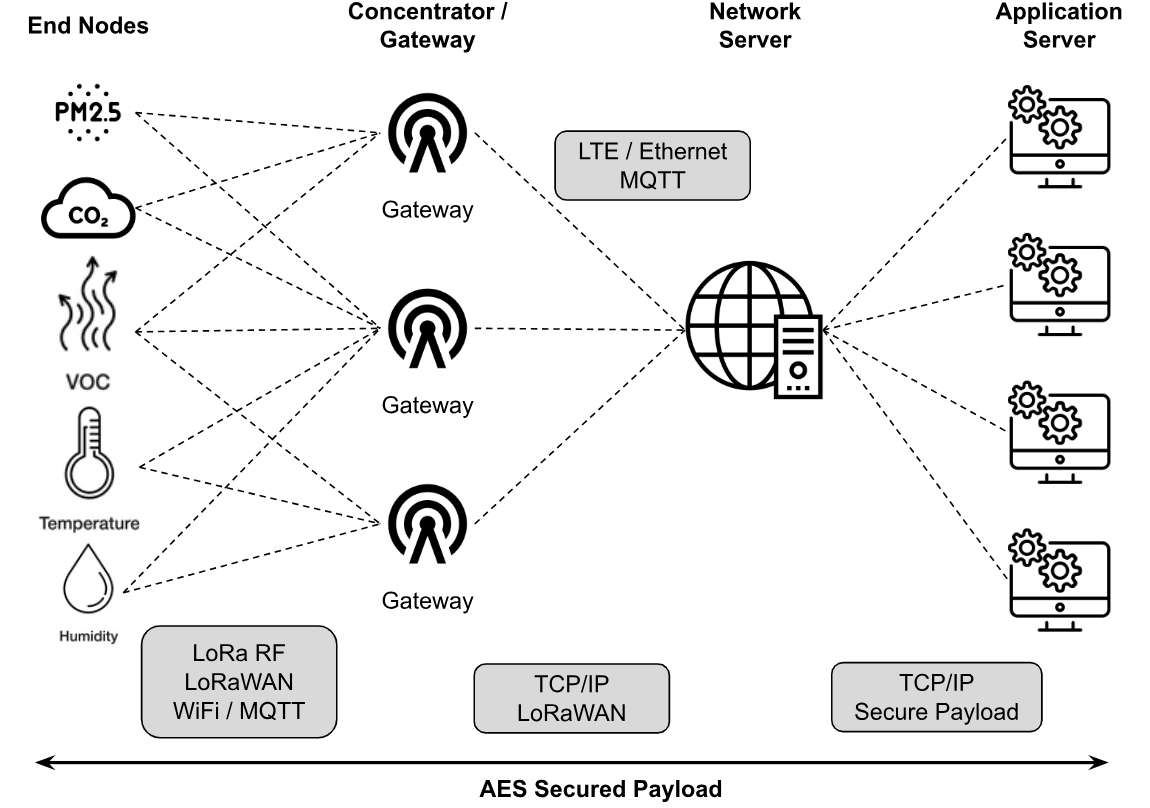
\includegraphics[width=.65\textwidth]{./Figuras/fig_1-diagBloques.png}
\caption{Diagrama en bloques del sistema.}
\label{fig:diagBloques}
\end{figure}

Este proyecto está diseñado como una solución adaptable, principalmente para implementarse en empresas, con la capacidad de escalar a hogares y gobierno. Todos los usuarios comparten una preocupación en común: la calidad del aire y su impacto en la salud. El sistema no solo permite el monitoreo en tiempo real, sino también envía alertas cuando los niveles de contaminación superan los límites recomendados. También ofrece herramientas para analizar datos históricos e identificar tendencias, que permitan tomar decisiones oportunas. Más que una simple innovación tecnológica, este proyecto representa una herramienta clave para mejorar la calidad de vida y promover un entorno más saludable y sostenible.

En el mercado actual existen soluciones para el monitoreo de la calidad del aire, sin embargo, muchas de ellas presentan limitaciones, como ser:
\begin{itemize}
	\item Costos elevados, en las etapas de implementación y mantenimiento, un sistema con carácteristicas similares puede volverse solo accesible a instituciones con grandes presupuestos.
	\item Cobertura limitada, ya que la mayoría de los sensores requieren cableado o dependencias de redes WiFi con alcance reducido.
	\item Falta de integración con plataformas acceesibles, lo que dificulta el análisis y la interpretación de los datos por parte de usuarios sin conocimientos técnicos avanzados.
\end{itemize}

A diferencia de estas soluciones, este proyeto esrtará diseñado como una solución flexible y adaptable a  empresas, hogares y gobiernos. Su propuesta de valor se basa en ofrecer un monitoreo ambiental accesible, para lograr entornos seguros y sostenibles, bajo los siguientes aspectos:

\begin{itemize}
	\item \textbf{Accesibilidad:} Una solución asequible en comparación con otros sistemas comerciales.
	\item \textbf{Escalabilidad:} Implementación modular, adaptable a distintos entornos y necesidades.
	\item \textbf{Interfaz intuitiva:} Plataforma accesible para cualquier usuario, sin necesidad de conocimientos técnicos avanzados.
	\item \textbf{Conectividad eficiente:} Uso de tecnologías de comunicación de bajo consumo y gran alcance.
	\item \textbf{Toma de decisiones informada:} Alertas y análisis de datos para implementar medidas de mitigación de contaminación.
\end{itemize}

El proyecto se encuentra en una etapa inicial de desarrollo, y para su primera versión se plantea una solución funcional, enfocada en validar su desempeño en entornos reales. En esta fase, el sistema ofrecerá dos modalidades de monitoreo que permitirán a los usuarios gestionar sus dispositivos de manera flexible:  

\begin{itemize}
    \item \textbf{Monitoreo privado:} Cada usuario podrá registrar y gestionar sus propios dispositivos, accediendo a la información en tiempo real de los sensores vinculados.  
    \item \textbf{Monitoreo público:} Si el usuario así lo decide, podrá compartir los datos recopilados con la comunidad, permitiendo que la información esté disponible en una red abierta. Esto fomentará la creación de un ecosistema colaborativo.  
\end{itemize}

En esta primera versión, no se implementarán modelos de suscripción, ni esquemas de pago, ya que el objetivo principal es desarrollar un prototipo funcional. Este proyecto permitaraá evaluar la viabilidad técnica y el impacto del sistema en distintos escenarios de uso.  

A futuro, se prevé la integración de herramientas más avanzadas, como modelos de análisis predictivo basados en inteligencia artificial y funcionalidades adicionales para mejorar la toma de decisiones en entornos urbanos e industriales. Con esta estrategia de crecimiento progresivo, el proyecto busca garantizar una implementación accesible y escalable, permitiendo que cada vez más usuarios se beneficien de un monitoreo ambiental confiable desde su primera versión.



\vspace{25px}


\section{2. Identificación y análisis de los interesados}
\label{sec:interesados}

\begin{table}[ht]
%\caption{Identificación de los interesados}
%\label{tab:interesados}
\begin{tabularx}{\linewidth}{@{}|l|X|X|l|@{}}
\hline
\rowcolor[HTML]{C0C0C0} 
Rol           & Nombre y Apellido & Organización 	& Puesto 	\\ \hline
Auspiciante   & -                 & -             	& -       	\\ \hline
Cliente       & \clientename      &\empclientename	&        	\\ \hline
Impulsor      & -                 & -             	& -       	\\ \hline
Responsable   & \authorname       & FIUBA        	& Alumno 	\\ \hline
Colaboradores & -                 & -             	& -       	\\ \hline
Orientador    & \supname	      & \pertesupname 	& Director del Trabajo Final \\ \hline
Equipo        & -                 & -             	& -       	\\ \hline
\end{tabularx}
\end{table}


\section{3. Propósito del proyecto}
\label{sec:proposito}

El propósito de este proyecto es fomentar entornos más saludables, seguros y sostenibles en zonas urbanas e industriales, mejorando la calidad del aire. Esto se logrará mediante un sistema de monitoreo basado en IoT, permitiendo recopilar, analizar y visualizar datos ambientales en tiempo real. Con esta herramienta, se busca facilitar la identificación de fuentes de contaminación y alertar para que las partes interesadas tomen acciones correctivas oportunas. Además, la solución ha sido diseñada para ser escalable, accesible y eficiente, asegurando su adaptabilidad a distintos entornos y necesidades.

\section{4. Alcance del proyecto}
\label{sec:alcance}

Este proyecto abarca el desarrollo e implementación de un sistema de monitoreo de calidad del aire basado en IoT. El sistema será capáz de medir (recolectar), transmitir, almacenar y mostrar datos en tiempo real, proporcionando información clave para la toma de deciciones.

El proyecto incluye:

\textbf{Dispositivos IoT (Nodos de Sensores)}
\begin{itemize}
	\item Microcontrolador: ESP32-S3 (por su conectividad WiFi/BLE, bajo consumo y módulo LoRa con antena incluido).
	\item Sensores:
	\begin{itemize}
		\item PM2.5/PM10: Sensor SDS011 o PMS5003 (mide partículas en suspensión).
		\item CO2: Sensor MH-Z19B o SCD30 (mide dióxido de carbono).
		\item VOCs: Sensor CCS811 o SGP30 (detecta compuestos orgánicos volátiles).
		\item Temperatura y Humedad: DHT22 o BME280.
	\end{itemize}

	\item Comunicación:
	\begin{itemize}
		\item LoRaWAN para áreas extensas (ej: ciudades) o WiFi/MQTT para interiores.
		\item Protocolo MQTT para enviar datos al servidor.
		\item Módulo Lora Sx1262 (incluido en el ESP32 de Heltec).
	\end{itemize}

	\item Alimentación: Batería recargable o USB (interiores).
\end{itemize}

\textbf{Servidor y Almacenamiento de Datos}
\begin{itemize}

	\item Protocolo de recepción: MQTT (usando brokers como Mosquitto, AWS IoT Core).
	
	\item Base de datos:
	\begin{itemize}
		\item Time-Series Database: InfluxDB (optimizada para datos temporales como lecturas de sensores).
		\item SQL/NoSQL: PostgreSQL o MongoDB (para consultas complejas).	
	\end{itemize}
	
	\item Procesamiento inicial:
	\begin{itemize}
		\item Validación de datos (eliminar valores atípicos).
		\item Normalización de unidades (ej: convertir ppm de CO2 a mg/m³).
	\end{itemize}

\end{itemize}

\textbf{Aplicativo Web/Móvil}
\begin{itemize}
	\item Frontend:
	\begin{itemize}
		\item Framework: React.js o Vue.js para dashboards interactivos.
		\item Librerías de visualización: Chart.js, D3.js o Grafana integrado.
	\end{itemize}
	
	\item Backend:
	\begin{itemize}
		\item API REST: Desarrollada en Node.js o Python (Django/Flask).
		\item Autenticación: JWT o OAuth2 para acceso seguro.
	\end{itemize}
	
	\item Características del aplicativo:
	\begin{itemize}
		\item Mapa en tiempo real con colores según el índice de calidad del aire.
		\item Gráficos históricos (tendencias de PM2.5, CO2, etc.).
		\item Alertas personalizables (notificaciones push).
		\item Descarga de informes en PDF/CSV. (deseado)	
	\end{itemize}		
	
\end{itemize}

\textbf{Flujo de Datos}
\begin{itemize}
	\item Recolección: Los sensores capturan datos cada 1-5 minutos.
	\item Transmisión: El ESP32 envía los datos vía MQTT/LoRaWAN al broker.
	\item Almacenamiento: El servidor procesa y guarda los datos en InfluxDB.
	\item Visualización: El aplicativo web consulta la API para mostrar datos en dashboards.
\end{itemize}

El presente proyecto no incluye:
\begin{itemize}
	\item Desarrollo de modelos de suscripción o monetización, ya que en esta fase el enfoque es la validación del prototipo.
	\item Integración con inteligencia artificial o modelos predictivos avanzados.
	\item Implementación de una red de sensores a gran escala más allá del piloto inicial.
	\item Certificaciones oficiales de calidad del aire, ya que el sistema servirá como referencia complementaria a mediciones gubernamentales o institucionales.
\end{itemize}

El alcance del proyecto está limitado a ser considerado un prototipo, enfocado en validar la viabilidad técnica y operativa. Las futuras versiones podrán incorporar mejoras basadas en los resultados de esta etapa.

\section{5. Supuestos del proyecto}
\label{sec:supuestos}

Para el desarrollo del presente proyecto se supone que:

\begin{itemize}
	\item \textbf{Disponibilidad financiera:} Dado que se trata de un emprendimiento personal, los costos del proyecto serán cubiertos por el responsable del proyecto.
	\item \textbf{Disponibilidad tecnológica:} Se cuenta con acceso a los sensores, microcontroladores y todos los componentes necesarios para la fabricación de los dispositovos IoT.
	\item \textbf{Factibilidad técnica:} Se asume que el diseño e implementación del sistema representa un reto que es el resultado de poner en práctica de lo aprendido en la especialización en IoT de la Universidad de Buenos Aires.
	\item \textbf{Tiempo:} El responsable debe cumplir con su planificación a ser propuesta, evitando retrasos y culminando el proyecto de manera satisfactoria.
	\item \textbf{Infraestructura de comunicación:} Se realizarán pruebas en entornos controlados asegurando que se cumple con la cobertura de la red LoRaWAN. En el caso de entornos cerrados se verificara la transmisión estable mediante WiFi/MQTT. De esta manera se asegura que los datos sean enviados para su visualización en línea, gracias al internet.
	\item \textbf{Consideración como prototipo:} En esta primera versión, el sistema se desarrollará como un prototipo funcional, con el objetivo de validar su desempeño y detectar oportunidades de mejora.
	\item \textbf{Aceptación del usuario:} Se espera que empresas, ciudadanos, ONGs y gobiernos muestren interes en utilizar la plataforma, incentivando un modelo de monitoreo colaborativo de la calidad del aire.

\end{itemize}

\section{6. Requerimientos}
\label{sec:requerimientos}

\begin{consigna}{red} % ELIMINAR \begin{consigna}{red} y \end{consigna}{red} en las secciones que vayan completando para cada entrega parcial.
Los requerimientos deben enumerarse y de ser posible estar agrupados por afinidad, por ejemplo:

\begin{enumerate}
	\item Requerimientos funcionales:
		\begin{enumerate}
			\item El sistema debe...
			\item Tal componente debe...
			\item El usuario debe poder...
		\end{enumerate}
	\item Requerimientos de documentación:
		\begin{enumerate}
			\item Requerimiento 1.
			\item Requerimiento 2 (prioridad menor)
		\end{enumerate}
	\item Requerimiento de testing...
	\item Requerimientos de la interfaz...
	\item Requerimientos interoperabilidad...
	\item etc...
\end{enumerate}

Leyendo los requerimientos se debe poder interpretar cómo será el proyecto y su funcionalidad.

Indicar claramente cuál es la prioridad entre los distintos requerimientos y si hay requerimientos opcionales. 

\textbf{¡¡¡No olvidarse de que los requerimientos incluyen a las regulaciones y normas vigentes!!!}

Y al escribirlos seguir las siguientes reglas:
\begin{itemize}
	\item Ser breve y conciso (nadie lee cosas largas). 
	\item Ser específico: no dejar lugar a confusiones.
	\item Expresar los requerimientos en términos que sean cuantificables y medibles.
\end{itemize}

\end{consigna} % ELIMINAR \begin{consigna}{red} y \end{consigna}{red} en las secciones que vayan completando para cada entrega parcial.

\section{7. Historias de usuarios (\textit{Product backlog})}
\label{sec:backlog}

\begin{consigna}{red}
Descripción: en esta sección se deben incluir las historias de usuarios y su ponderación (\textit{history points}). Recordar que las historias de usuarios son descripciones cortas y simples de una característica contada desde la perspectiva de la persona que desea la nueva capacidad, generalmente un usuario o cliente del sistema. La ponderación es un número entero que representa el tamaño de la historia comparada con otras historias de similar tipo.

Se debe indicar explícitamente el criterio para calcular los \textit{story points} de cada historia.

El formato propuesto es: 
\begin{enumerate}
\item ``Como [rol] quiero [tal cosa] para [tal otra cosa]."

\textit{Story points}: 8 (complejidad: 3, dificultad: 2, incertidumbre: 3)
\end{enumerate}
\end{consigna}

\section{8. Entregables principales del proyecto}
\label{sec:entregables}

\begin{consigna}{red}
Los entregables del proyecto son (ejemplo):

\begin{itemize}
	\item Manual de usuario.
	\item Diagrama de circuitos esquemáticos.
	\item Código fuente del firmware.
	\item Diagrama de instalación.
	\item Memoria del trabajo final.
	\item etc...
\end{itemize}
\end{consigna}

\section{9. Desglose del trabajo en tareas}
\label{sec:wbs}

\begin{consigna}{red}
El WBS debe tener relación directa o indirecta con los requerimientos.  Son todas las actividades que se harán en el proyecto para dar cumplimiento a los requerimientos. Se recomienda mostrar el WBS mediante una lista indexada:

\begin{enumerate}
\item Grupo de tareas 1 (suma h)
	\begin{enumerate}
	\item Tarea 1 (tantas h)
	\item Tarea 2 (tantas h)
	\item Tarea 3 (tantas h)
	\end{enumerate}
\item Grupo de tareas 2 (suma h)
	\begin{enumerate}
	\item Tarea 1 (tantas h)
	\item Tarea 2 (tantas h)
	\item Tarea 3 (tantas h)
	\end{enumerate}
\item Grupo de tareas 3 (suma h)
	\begin{enumerate}
	\item Tarea 1 (tantas h)
	\item Tarea 2 (tantas h)
	\item Tarea 3 (tantas h)
	\item Tarea 4 (tantas h)
	\item Tarea 5 (tantas h)
	\end{enumerate}
\end{enumerate}

Cantidad total de horas: tantas.

\textbf{¡Importante!:} la unidad de horas es h y va separada por espacio del número. Es incorrecto escribir ``23hs".

\textbf{Se recomienda que no haya ninguna tarea que lleve más de 40 h.} De ser así se recomienda dividirla en tareas de menor duración.

\end{consigna}

\section{10. Diagrama de Activity On Node}
\label{sec:AoN}

\begin{consigna}{red}
Armar el AoN a partir del WBS definido en la etapa anterior.

Una herramienta simple para desarrollar los diagramas es el Draw.io (\url{https://app.diagrams.net/}).
\href{https://app.diagrams.net}{Draw.io}


\begin{figure}[htpb]
\centering 
\includegraphics[width=.8\textwidth]{./Figuras/AoN.png}
\caption{Diagrama de \textit{Activity on Node}.}
\label{fig:AoN}
\end{figure}

Indicar claramente en qué unidades están expresados los tiempos.
De ser necesario indicar los caminos semi críticos y analizar sus tiempos mediante un cuadro.
Es recomendable usar colores y un cuadro indicativo describiendo qué representa cada color.

\end{consigna}

\section{11. Diagrama de Gantt}
\label{sec:gantt}

\begin{consigna}{red}
Existen muchos programas y recursos \textit{online} para hacer diagramas de Gantt, entre los cuales destacamos:

\begin{itemize}
\item Planner
\item GanttProject
\item Trello + \textit{plugins}. En el siguiente link hay un tutorial oficial: \\ \url{https://blog.trello.com/es/diagrama-de-gantt-de-un-proyecto}
\item Creately, herramienta online colaborativa. \\\url{https://creately.com/diagram/example/ieb3p3ml/LaTeX}
\item Se puede hacer en latex con el paquete \textit{pgfgantt}\\ \url{http://ctan.dcc.uchile.cl/graphics/pgf/contrib/pgfgantt/pgfgantt.pdf}
\end{itemize}

Pegar acá una captura de pantalla del diagrama de Gantt, cuidando que la letra sea suficientemente grande como para ser legible. 
Si el diagrama queda demasiado ancho, se puede pegar primero la ``tabla'' del Gantt y luego pegar la parte del diagrama de barras del diagrama de Gantt.

Configurar el software para que en la parte de la tabla muestre los códigos del EDT (WBS).\\
Configurar el software para que al lado de cada barra muestre el nombre de cada tarea.\\
Revisar que la fecha de finalización coincida con lo indicado en el Acta Constitutiva.

En la figura \ref{fig:gantt}, se muestra un ejemplo de diagrama de gantt realizado con el paquete de \textit{pgfgantt}. 
En la plantilla pueden ver el código que lo genera y usarlo de base para construir el propio.

Las fechas pueden ser calculadas utilizando alguna de las herramientas antes citadas. Sin embargo, el siguiente ejemplo
fue elaborado utilizando 
\href{https://docs.google.com/spreadsheets/d/1fBz8NhSpc4tkkhz3KjJCbh1nR_ltDkfEcZi4tZXduqs}{esta hoja de cálculo}.

Es importante destacar que el ancho del diagrama estará dado por la longitud del texto utilizado para las tareas 
(Ejemplo: tarea 1, tarea 2, etcétera) y el valor \textit{x unit}. Para mejorar la apariencia del diagrama, es necesario
ajustar este valor y, quizás, acortar los nombres de las tareas.

\begin{figure}[htpb]
  \begin{center}
    \begin{ganttchart}[
      time slot unit=day,
      time slot format=isodate,
      x unit=0.038cm,
      y unit title=0.7cm,
      y unit chart=0.6cm,
      milestone/.append style={xscale=4}
      ]{2021-03-05}{2021-12-16}
      \gantttitlecalendar*{2021-03-05}{2021-12-16}{year} \\
      \gantttitlecalendar*{2021-03-05}{2021-12-16}{month} \\
      \ganttgroup{Duración Total}{2021-03-05}{2021-12-16} \\
      %%%%%%%%%%%%%%%%%Organización
      \ganttgroup{Organización}{2021-03-05}{2021-04-16} \\
      \ganttbar{Planificación del proyecto}{2021-03-05}{2021-04-15} \\
      %%%%%%%%%%%%%%%%%Ejecución
      \ganttgroup{Ejecución}{2021-04-16}{2021-10-21} \\
      \ganttbar{Tarea 1}{2021-04-16}{2021-04-29} \\
      \ganttbar{Tarea 2}{2021-04-30}{2021-05-13} \\
      \ganttbar{Tarea 3}{2021-05-14}{2021-05-27} \\
      \ganttbar{Tarea 4}{2021-05-28}{2021-07-12} \\
      \ganttbar{Tarea 5}{2021-07-13}{2021-08-09} \\
      \ganttbar{Tarea 6}{2021-08-10}{2021-09-23} \\
      \ganttbar{Tarea 7}{2021-09-24}{2021-09-30} \\
      \ganttbar{Tarea 8}{2021-10-01}{2021-10-14} \\
      \ganttbar{Tarea 9}{2021-10-15}{2021-10-21} \\
      % %%%%%%%%%%%%%%%%%Finalización
      \ganttgroup{Finalización}{2021-10-22}{2021-12-16} \\
      \ganttbar{Memoria v1}{2021-10-22}{2021-11-04} \\
      \ganttbar{Memoria v2}{2021-11-05}{2021-11-18} \\
      \ganttbar{Memoria final}{2021-11-19}{2021-12-02} \\
      % La fecha del siguiente milestone es la fecha en que terminamos la memoria
      \ganttmilestone{Enviar memoria al director}{2021-12-02} \\
      \ganttbar{Elaborar la presentación}{2021-12-03}{2021-12-16} \\
      \ganttmilestone{Ensayo de la presentación}{2021-12-16} \\
      %%%%%%%%%%%%%%%%%%%%%%%%%%%%%%%%%%%%%%%%%%%%%%%%%%%%%%%%%%%%%%%
    \end{ganttchart}
  \end{center}
  \caption{Diagrama de gantt de ejemplo}
  \label{fig:gantt}
\end{figure}


\begin{landscape}
\begin{figure}[htpb]
\centering 
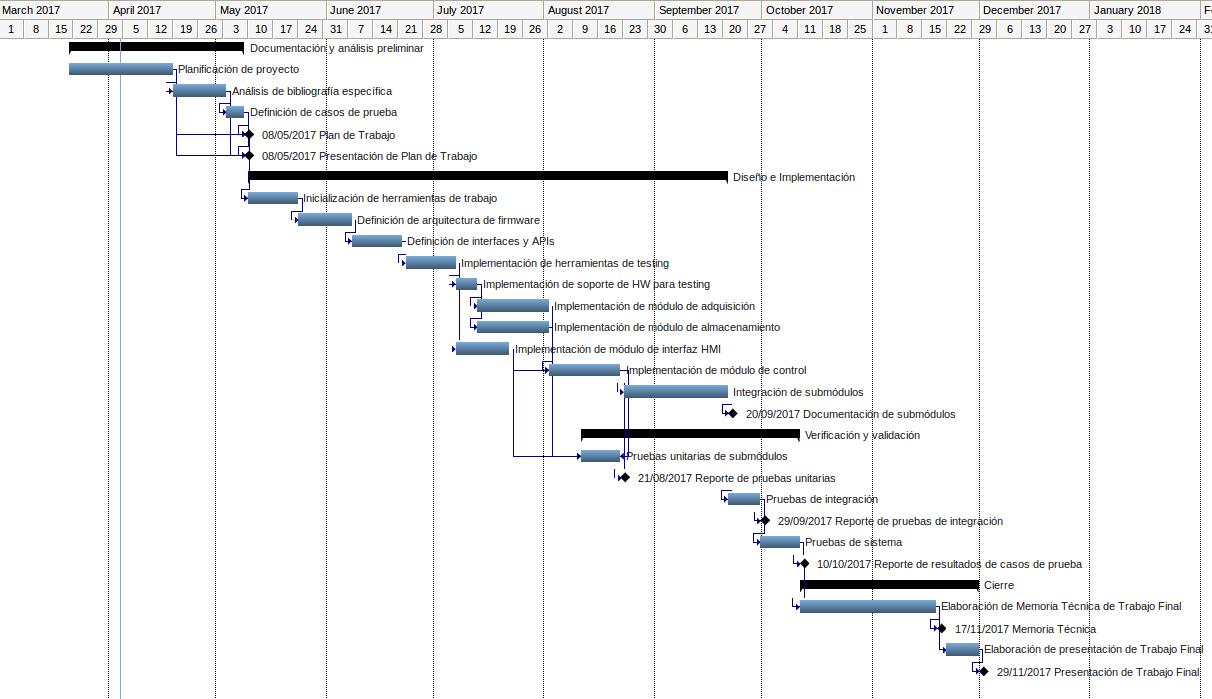
\includegraphics[height=.85\textheight]{./Figuras/Gantt-2.png}
\caption{Ejemplo de diagrama de Gantt (apaisado).} %Modificar este título acorde.
\label{fig:diagGantt}
\end{figure}

\end{landscape}

\end{consigna}


\section{12. Presupuesto detallado del proyecto}
\label{sec:presupuesto}

\begin{consigna}{red}
Si el proyecto es complejo entonces separarlo en partes:
\begin{itemize}
	\item Un total global, indicando el subtotal acumulado por cada una de las áreas.
	\item El desglose detallado del subtotal de cada una de las áreas.
\end{itemize}

IMPORTANTE: No olvidarse de considerar los COSTOS INDIRECTOS.

Incluir la aclaración de si se emplea como moneda el peso argentino (ARS) o si se usa moneda extranjera (USD, EUR, etc). Si es en moneda extranjera se debe indicar la tasa de conversión respecto a la moneda local en una fecha dada.

\end{consigna}

\begin{table}[htpb]
\centering
\begin{tabularx}{\linewidth}{@{}|X|c|r|r|@{}}
\hline
\rowcolor[HTML]{C0C0C0} 
\multicolumn{4}{|c|}{\cellcolor[HTML]{C0C0C0}COSTOS DIRECTOS} \\ \hline
\rowcolor[HTML]{C0C0C0} 
Descripción &
  \multicolumn{1}{c|}{\cellcolor[HTML]{C0C0C0}Cantidad} &
  \multicolumn{1}{c|}{\cellcolor[HTML]{C0C0C0}Valor unitario} &
  \multicolumn{1}{c|}{\cellcolor[HTML]{C0C0C0}Valor total} \\ \hline
 &
  \multicolumn{1}{c|}{} &
  \multicolumn{1}{c|}{} &
  \multicolumn{1}{c|}{} \\ \hline
 &
  \multicolumn{1}{c|}{} &
  \multicolumn{1}{c|}{} &
  \multicolumn{1}{c|}{} \\ \hline
\multicolumn{1}{|l|}{} &
   &
   &
   \\ \hline
\multicolumn{1}{|l|}{} &
   &
   &
   \\ \hline
\multicolumn{3}{|c|}{SUBTOTAL} &
  \multicolumn{1}{c|}{} \\ \hline
\rowcolor[HTML]{C0C0C0} 
\multicolumn{4}{|c|}{\cellcolor[HTML]{C0C0C0}COSTOS INDIRECTOS} \\ \hline
\rowcolor[HTML]{C0C0C0} 
Descripción &
  \multicolumn{1}{c|}{\cellcolor[HTML]{C0C0C0}Cantidad} &
  \multicolumn{1}{c|}{\cellcolor[HTML]{C0C0C0}Valor unitario} &
  \multicolumn{1}{c|}{\cellcolor[HTML]{C0C0C0}Valor total} \\ \hline
\multicolumn{1}{|l|}{} &
   &
   &
   \\ \hline
\multicolumn{1}{|l|}{} &
   &
   &
   \\ \hline
\multicolumn{1}{|l|}{} &
   &
   &
   \\ \hline
\multicolumn{3}{|c|}{SUBTOTAL} &
  \multicolumn{1}{c|}{} \\ \hline
\rowcolor[HTML]{C0C0C0}
\multicolumn{3}{|c|}{TOTAL} &
   \\ \hline
\end{tabularx}%
\end{table}


\section{13. Gestión de riesgos}
\label{sec:riesgos}

\begin{consigna}{red}
a) Identificación de los riesgos (al menos cinco) y estimación de sus consecuencias:
 
Riesgo 1: detallar el riesgo (riesgo es algo que si ocurre altera los planes previstos de forma negativa)
\begin{itemize}
	\item Severidad (S): mientras más severo, más alto es el número (usar números del 1 al 10).\\
	Justificar el motivo por el cual se asigna determinado número de severidad (S).
	\item Probabilidad de ocurrencia (O): mientras más probable, más alto es el número (usar del 1 al 10).\\
	Justificar el motivo por el cual se asigna determinado número de (O). 
\end{itemize}   

Riesgo 2:
\begin{itemize}
	\item Severidad (S): X.\\
	Justificación...
	\item Ocurrencia (O): Y.\\
	Justificación...
\end{itemize}

Riesgo 3:
\begin{itemize}
	\item Severidad (S):  X.\\
	Justificación...
	\item Ocurrencia (O): Y.\\
	Justificación...
\end{itemize}


b) Tabla de gestión de riesgos:      (El RPN se calcula como RPN=SxO)

\begin{table}[htpb]
\centering
\begin{tabularx}{\linewidth}{@{}|X|c|c|c|c|c|c|@{}}
\hline
\rowcolor[HTML]{C0C0C0} 
Riesgo & S & O & RPN & S* & O* & RPN* \\ \hline
       &   &   &     &    &    &      \\ \hline
       &   &   &     &    &    &      \\ \hline
       &   &   &     &    &    &      \\ \hline
       &   &   &     &    &    &      \\ \hline
       &   &   &     &    &    &      \\ \hline
\end{tabularx}%
\end{table}

Criterio adoptado: 

Se tomarán medidas de mitigación en los riesgos cuyos números de RPN sean mayores a...

Nota: los valores marcados con (*) en la tabla corresponden luego de haber aplicado la mitigación.

c) Plan de mitigación de los riesgos que originalmente excedían el RPN máximo establecido:
 
Riesgo 1: plan de mitigación (si por el RPN fuera necesario elaborar un plan de mitigación).
  Nueva asignación de S y O, con su respectiva justificación:
  \begin{itemize}
	\item Severidad (S*): mientras más severo, más alto es el número (usar números del 1 al 10).
          Justificar el motivo por el cual se asigna determinado número de severidad (S).
	\item Probabilidad de ocurrencia (O*): mientras más probable, más alto es el número (usar del 1 al 10).
          Justificar el motivo por el cual se asigna determinado número de (O).
	\end{itemize}

Riesgo 2: plan de mitigación (si por el RPN fuera necesario elaborar un plan de mitigación).
 
Riesgo 3: plan de mitigación (si por el RPN fuera necesario elaborar un plan de mitigación).

\end{consigna}


\section{14. Gestión de la calidad}
\label{sec:calidad}

\begin{consigna}{red}
Elija al menos diez requerimientos que a su criterio sean los más importantes/críticos/que aportan más valor y para cada uno de ellos indique las acciones de verificación y validación que permitan asegurar su cumplimiento.

\begin{itemize} 
\item Req \#1: copiar acá el requerimiento con su correspondiente número.

\begin{itemize}
	\item Verificación para confirmar si se cumplió con lo requerido antes de mostrar el sistema al cliente. Detallar.
	\item Validación con el cliente para confirmar que está de acuerdo en que se cumplió con lo requerido. Detallar. 
\end{itemize}

\end{itemize}

Tener en cuenta que en este contexto se pueden mencionar simulaciones, cálculos, revisión de hojas de datos, consulta con expertos, mediciones, etc.  

Las acciones de verificación suelen considerar al entregable como ``caja blanca'', es decir se conoce en profundidad su funcionamiento interno.  

En cambio, las acciones de validación suelen considerar al entregable como ``caja negra'', es decir, que no se conocen los detalles de su funcionamiento interno.

\end{consigna}

\section{15. Procesos de cierre}    
\label{sec:cierre}

\begin{consigna}{red}
Establecer las pautas de trabajo para realizar una reunión final de evaluación del proyecto, tal que contemple las siguientes actividades:

\begin{itemize}
	\item Pautas de trabajo que se seguirán para analizar si se respetó el Plan de Proyecto original:\\
	 - Indicar quién se ocupará de hacer esto y cuál será el procedimiento a aplicar. 
	\item Identificación de las técnicas y procedimientos útiles e inútiles que se emplearon, los problemas que surgieron y cómo se solucionaron:\\
	 - Indicar quién se ocupará de hacer esto y cuál será el procedimiento para dejar registro.
	\item Indicar quién organizará el acto de agradecimiento a todos los interesados, y en especial al equipo de trabajo y colaboradores:\\
	  - Indicar esto y quién financiará los gastos correspondientes.
\end{itemize}

\end{consigna}

\end{document}